Předkládaná práce se zabývá jedním z magneto-optických experimentů probíhajících v Laboratoři OptoSpintroniky (LOS), společném pracovišti MFF UK a FZU AV ČR, na adrese Ke Karlovu 3, Praha 2.\todopn{je to dobře napsané?}

Zkráceně lze popsat jako \emph{spektroskopie anizotropních kvadratických MO jevů} (MLD/Voigtova/Cotton-Moutonova jevu) a přidružená \emph{in-plane magneto-metrie} tenkých feromagnetických filmů v téměř kolmém dopadu a rotujícím poli.
Schéma aparatury je na obr. \ref{fig:zakladni-schema}.
Následuje popis jednotlivých elementů

\begin{figure}[htbp]
    \centering
    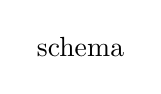
\begin{tikzpicture}
    \path (0,0) node {\missingfigure{schema}};
\end{tikzpicture}

    \caption{schema}
    \label{fig:zakladni-schema}
\end{figure}

\paragraph{Vektorový magnet}
Elektro-magnet tvořený dvěma páry nezávislých cívek dokáže vytvořit libovolné vnější magnetické pole $\vHext$ v rovině $xy$ o maximální velikosti \SI{210}{\milli\tesla}.
V praxi jsou kvůli hysterezi magnetu použity pouze definované charakterizované procedury (posloupnosti proudů).
Vývojem proudových tabulek se zabývá \cite{kimakCharakterizaciaDvojdimenzionalnehoElektromagnetu2017,kimakOptickaSpektroskopieAntiferomagnetu2019}.
V této práci používáme pouze dvě: rotaci pole o velikosti $\Hext=\SI{207}{\milli\tesla}, \SI{50}{\milli\tesla}$ s krokem v úhlu pole $\phih$ minimálně \SI{1}{\degree}.

\paragraph{Kryostat}
Kryostat s topením dovoluje udržovat vzorek v rozmezí teplot cca 15--\SI{800}{\kelvin}.
Vzorek je lepen na \emph{cold-finger} a v kryogenické komoře umístěn mezi ramena magnetu.
Komora je opatřena zpředu a ze stran skleněnými okénky.
Magneto-optickou aktivitu okének (Faradayův jev) zkoumá \cite{baduraMagnetooptickaMereniPro2019}.

\paragraph{Super-kontinuální laser}
\emph{SuperK EXTREME} generuje široko-spektrální pulzy, které jsou dále filtrovány pro získání pulzů s šířkou pásma \SI{10}{\nano\meter}.
V rozmezí \num{460}--\SI{845}{\nano\meter} k filtraci používáme laditelný filtr \emph{SuperK VARIA}, v rozmezí \num{845}--\SI{1600}{\nano\meter} pak sadu pásmových interferenčních filtrů.

\paragraph{Polarizační optika}
Pevně umístěné polarizatóry P0 a P2 jsou širokospektrální typu Glan Laser.
Polarizátor v motorizovaném rotačním držáku P1 je absorpční, daný rozsah vlnových délek je pokryt polarizátory s označením P-VIS (\num{0}--\SI{0}{\nano\meter})\todo{doplnit rozsahy} a P-IR (\num{0}--\SI{0}{\nano\meter}).
Půlvlnné destičky WP1, WP2 jsou také motorizované a vyskytují se ve třech sadách: VIS1, VIS2 (\num{0}--\SI{0}{\nano\meter}); NIR1, NIR2 (\num{0}--\SI{0}{\nano\meter}); IR1, IR2 (\num{0}--\SI{0}{\nano\meter}).

\subparagraph{PEM}
Foto-elastický modulátor (není na schématu) je zařízení, ve kterém vlivem zvukové vlny dochází k modulaci lineárního dvojlomu,
takže se chová jako retardér s periodicky modulovaným fázovým zpožděním (viz \eqref{eqn:cisty-retarder}) $\Delta(t) \propto \cos(\omega_\textrm{PEM}t)$. 

Charakterizaci a širšímu popisu se věnuje \cite{minarModulacePolarizaceSvetelne2004}.

\subparagraph{Berekův kompenzátor}
Berekův kompenzátor je retardér tvořený dvojlomným krystalem, jehož naklápěním lze dosáhnout libovolného (v daném rozsahu) fázového zpoždění $\Delta$ mezi kolmými lineárními polarizacemi.
Jedná se tedy o laditelný retardér (fázovou destičku).
Charakterizaci se věnuje \cite{schusserSkryteKouzloPolarizace2014}.

\paragraph{Detektory}
V rozsahu \num{460}--\SI{1100}{\nano\meter} používáme křemíkové diody.
V infračervené oblasti \num{1000}--\SI{1600}{\nano\meter} používáme detektory na bázi \ch{InGaAs}, které byly studovány v \cite{hovorakovaCharakterizaceInfracervenehoDetektoru}.

\paragraph{Optický můstek}
K měření je využito schéma optického můstku popsané v oddílu \ref{chap:mustek-kap2}.

\paragraph{Chopper}
Ve dráze svazku je vždy umístěn intenzitní modulátor (\emph{chopper}), který dovoluje přesnější měření pomocí fázově citlivých zesilovačů (\emph{lock-inů}).
